% Graphic for TeX using PGF
% Title: /home/jnicolaschc/GitHub/Metodología de la Investigación/enfoque_marco_logico/Esquemas/Árbol de Objetivos/pgf/arbolObjetivos.dia
% Creator: Dia v0.97+git
% CreationDate: Mon Aug 16 12:03:15 2021
% For: jnicolaschc
% \usepackage{tikz}
% The following commands are not supported in PSTricks at present
% We define them conditionally, so when they are implemented,
% this pgf file will use them.
\ifx\du\undefined
	\newlength{\du}
\fi
\setlength{\du}{15\unitlength}
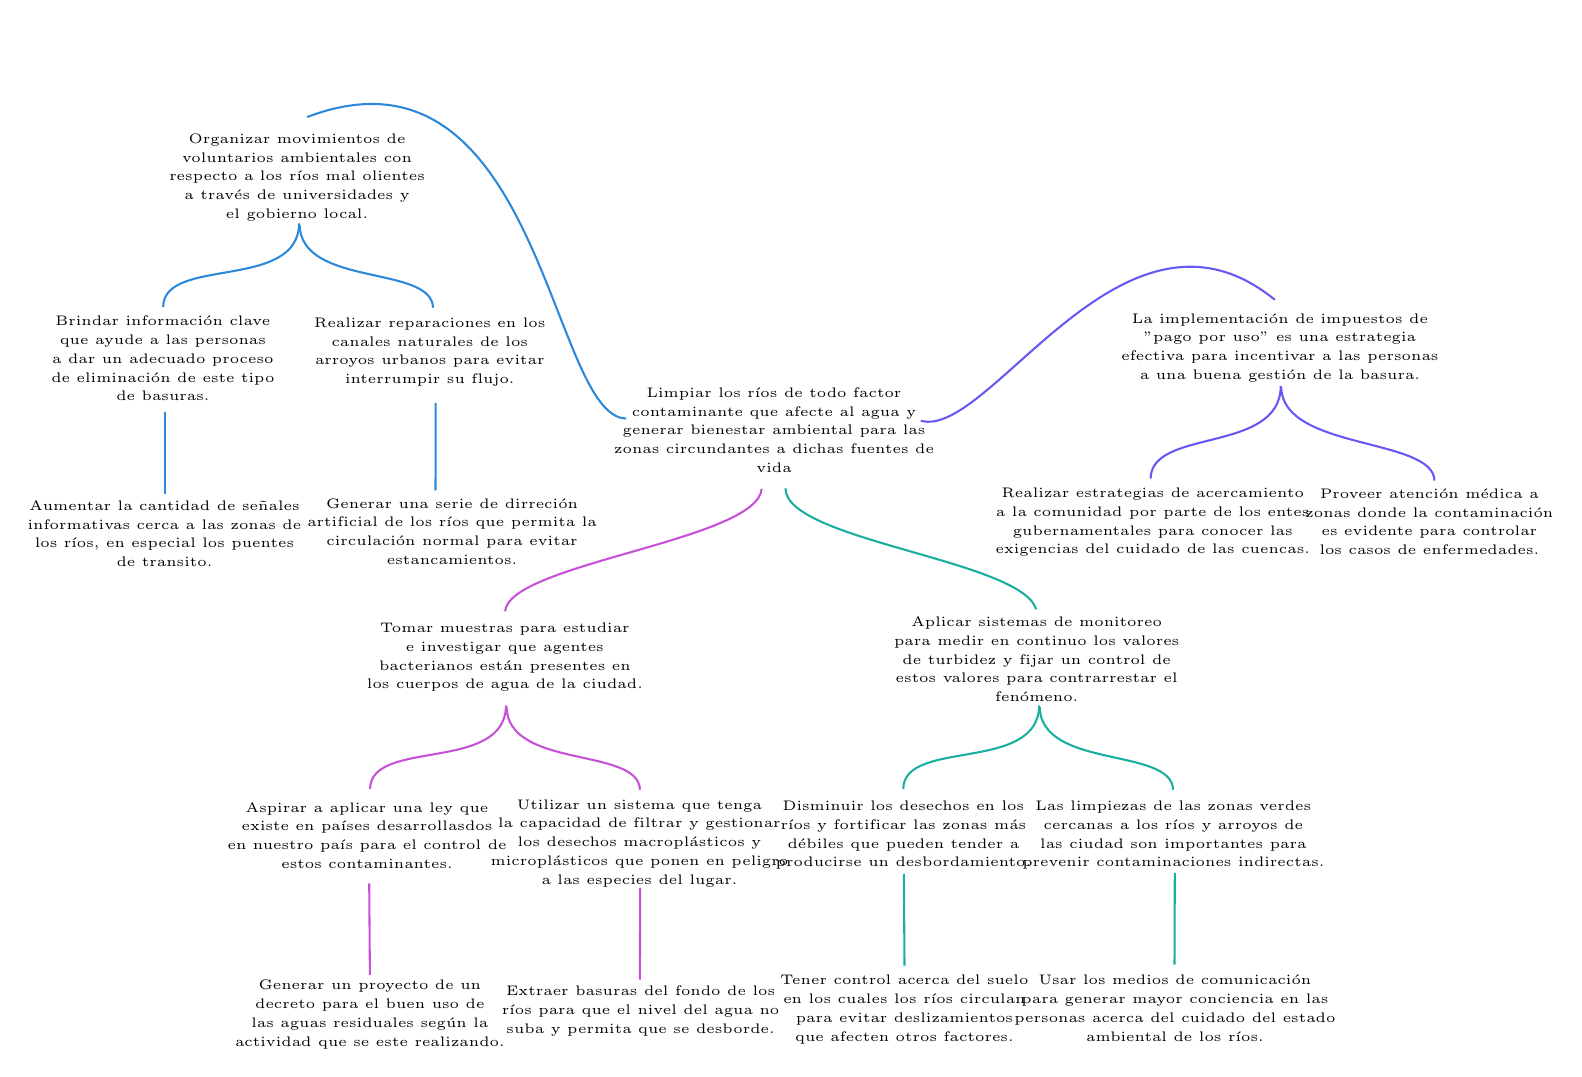
\begin{tikzpicture}[scale = 1.6]
	\pgftransformxscale{1.000000}
	\pgftransformyscale{-1.000000}
	\definecolor{dialinecolor}{rgb}{0.000000, 0.000000, 0.000000}
	\pgfsetstrokecolor{dialinecolor}
	\pgfsetstrokeopacity{1.000000}
	\definecolor{diafillcolor}{rgb}{1.000000, 1.000000, 1.000000}
	\pgfsetfillcolor{diafillcolor}
	\pgfsetfillopacity{1.000000}
	% setfont left to latex
	\definecolor{dialinecolor}{rgb}{0.000000, 0.000000, 0.000000}
	\pgfsetstrokecolor{dialinecolor}
	\pgfsetstrokeopacity{1.000000}
	\definecolor{diafillcolor}{rgb}{0.000000, 0.000000, 0.000000}
	\pgfsetfillcolor{diafillcolor}
	\pgfsetfillopacity{1.000000}
	\node[anchor=base,inner sep=0pt, outer sep=0pt,color=dialinecolor] at (2.042159\du,-11.237636\du){\tiny{Limpiar los ríos de todo factor}};
	% setfont left to latex
	\definecolor{dialinecolor}{rgb}{0.000000, 0.000000, 0.000000}
	\pgfsetstrokecolor{dialinecolor}
	\pgfsetstrokeopacity{1.000000}
	\definecolor{diafillcolor}{rgb}{0.000000, 0.000000, 0.000000}
	\pgfsetfillcolor{diafillcolor}
	\pgfsetfillopacity{1.000000}
	\node[anchor=base,inner sep=0pt, outer sep=0pt,color=dialinecolor] at (2.042159\du,-10.955414\du){\tiny{contaminante que afecte al agua y}};
	% setfont left to latex
	\definecolor{dialinecolor}{rgb}{0.000000, 0.000000, 0.000000}
	\pgfsetstrokecolor{dialinecolor}
	\pgfsetstrokeopacity{1.000000}
	\definecolor{diafillcolor}{rgb}{0.000000, 0.000000, 0.000000}
	\pgfsetfillcolor{diafillcolor}
	\pgfsetfillopacity{1.000000}
	\node[anchor=base,inner sep=0pt, outer sep=0pt,color=dialinecolor] at (2.042159\du,-10.673192\du){\tiny{generar bienestar ambiental para las}};
	% setfont left to latex
	\definecolor{dialinecolor}{rgb}{0.000000, 0.000000, 0.000000}
	\pgfsetstrokecolor{dialinecolor}
	\pgfsetstrokeopacity{1.000000}
	\definecolor{diafillcolor}{rgb}{0.000000, 0.000000, 0.000000}
	\pgfsetfillcolor{diafillcolor}
	\pgfsetfillopacity{1.000000}
	\node[anchor=base,inner sep=0pt, outer sep=0pt,color=dialinecolor] at (2.042159\du,-10.390970\du){\tiny{zonas circundantes a dichas fuentes de}};
	% setfont left to latex
	\definecolor{dialinecolor}{rgb}{0.000000, 0.000000, 0.000000}
	\pgfsetstrokecolor{dialinecolor}
	\pgfsetstrokeopacity{1.000000}
	\definecolor{diafillcolor}{rgb}{0.000000, 0.000000, 0.000000}
	\pgfsetfillcolor{diafillcolor}
	\pgfsetfillopacity{1.000000}
	\node[anchor=base,inner sep=0pt, outer sep=0pt,color=dialinecolor] at (2.042159\du,-10.108747\du){\tiny{vida}};
	% setfont left to latex
	\definecolor{dialinecolor}{rgb}{0.000000, 0.000000, 0.000000}
	\pgfsetstrokecolor{dialinecolor}
	\pgfsetstrokeopacity{1.000000}
	\definecolor{diafillcolor}{rgb}{0.000000, 0.000000, 0.000000}
	\pgfsetfillcolor{diafillcolor}
	\pgfsetfillopacity{1.000000}
	\node[anchor=base,inner sep=0pt, outer sep=0pt,color=dialinecolor] at (-5.139835\du,-15.063162\du){\tiny{Organizar movimientos de}};
	% setfont left to latex
	\definecolor{dialinecolor}{rgb}{0.000000, 0.000000, 0.000000}
	\pgfsetstrokecolor{dialinecolor}
	\pgfsetstrokeopacity{1.000000}
	\definecolor{diafillcolor}{rgb}{0.000000, 0.000000, 0.000000}
	\pgfsetfillcolor{diafillcolor}
	\pgfsetfillopacity{1.000000}
	\node[anchor=base,inner sep=0pt, outer sep=0pt,color=dialinecolor] at (-5.139835\du,-14.780940\du){\tiny{voluntarios ambientales con}};
	% setfont left to latex
	\definecolor{dialinecolor}{rgb}{0.000000, 0.000000, 0.000000}
	\pgfsetstrokecolor{dialinecolor}
	\pgfsetstrokeopacity{1.000000}
	\definecolor{diafillcolor}{rgb}{0.000000, 0.000000, 0.000000}
	\pgfsetfillcolor{diafillcolor}
	\pgfsetfillopacity{1.000000}
	\node[anchor=base,inner sep=0pt, outer sep=0pt,color=dialinecolor] at (-5.139835\du,-14.498717\du){\tiny{respecto a los ríos mal olientes}};
	% setfont left to latex
	\definecolor{dialinecolor}{rgb}{0.000000, 0.000000, 0.000000}
	\pgfsetstrokecolor{dialinecolor}
	\pgfsetstrokeopacity{1.000000}
	\definecolor{diafillcolor}{rgb}{0.000000, 0.000000, 0.000000}
	\pgfsetfillcolor{diafillcolor}
	\pgfsetfillopacity{1.000000}
	\node[anchor=base,inner sep=0pt, outer sep=0pt,color=dialinecolor] at (-5.139835\du,-14.216495\du){\tiny{a través de universidades y}};
	% setfont left to latex
	\definecolor{dialinecolor}{rgb}{0.000000, 0.000000, 0.000000}
	\pgfsetstrokecolor{dialinecolor}
	\pgfsetstrokeopacity{1.000000}
	\definecolor{diafillcolor}{rgb}{0.000000, 0.000000, 0.000000}
	\pgfsetfillcolor{diafillcolor}
	\pgfsetfillopacity{1.000000}
	\node[anchor=base,inner sep=0pt, outer sep=0pt,color=dialinecolor] at (-5.139835\du,-13.934273\du){\tiny{el gobierno local.}};
	\pgfsetlinewidth{0.050000\du}
	\pgfsetdash{}{0pt}
	\pgfsetmiterjoin
	\pgfsetbuttcap
	{
		\definecolor{diafillcolor}{rgb}{0.172549, 0.533333, 0.850980}
		\pgfsetfillcolor{diafillcolor}
		\pgfsetfillopacity{1.000000}
		% was here!!!
		\definecolor{dialinecolor}{rgb}{0.172549, 0.533333, 0.850980}
		\pgfsetstrokecolor{dialinecolor}
		\pgfsetstrokeopacity{1.000000}
		\pgfpathmoveto{\pgfpoint{-0.184604\du}{-10.920245\du}}
		\pgfpathcurveto{\pgfpoint{-1.330841\du}{-10.931707\du}}{\pgfpoint{-1.479852\du}{-16.788978\du}}{\pgfpoint{-4.987337\du}{-15.459343\du}}
		\pgfusepath{stroke}
	}
	% setfont left to latex
	\definecolor{dialinecolor}{rgb}{0.000000, 0.000000, 0.000000}
	\pgfsetstrokecolor{dialinecolor}
	\pgfsetstrokeopacity{1.000000}
	\definecolor{diafillcolor}{rgb}{0.000000, 0.000000, 0.000000}
	\pgfsetfillcolor{diafillcolor}
	\pgfsetfillopacity{1.000000}
	\node[anchor=base,inner sep=0pt, outer sep=0pt,color=dialinecolor] at (-7.159953\du,-12.314161\du){\tiny{Brindar información clave}};
	% setfont left to latex
	\definecolor{dialinecolor}{rgb}{0.000000, 0.000000, 0.000000}
	\pgfsetstrokecolor{dialinecolor}
	\pgfsetstrokeopacity{1.000000}
	\definecolor{diafillcolor}{rgb}{0.000000, 0.000000, 0.000000}
	\pgfsetfillcolor{diafillcolor}
	\pgfsetfillopacity{1.000000}
	\node[anchor=base,inner sep=0pt, outer sep=0pt,color=dialinecolor] at (-7.159953\du,-12.031939\du){\tiny{que ayude a las personas}};
	% setfont left to latex
	\definecolor{dialinecolor}{rgb}{0.000000, 0.000000, 0.000000}
	\pgfsetstrokecolor{dialinecolor}
	\pgfsetstrokeopacity{1.000000}
	\definecolor{diafillcolor}{rgb}{0.000000, 0.000000, 0.000000}
	\pgfsetfillcolor{diafillcolor}
	\pgfsetfillopacity{1.000000}
	\node[anchor=base,inner sep=0pt, outer sep=0pt,color=dialinecolor] at (-7.159953\du,-11.749717\du){\tiny{a dar un adecuado proceso}};
	% setfont left to latex
	\definecolor{dialinecolor}{rgb}{0.000000, 0.000000, 0.000000}
	\pgfsetstrokecolor{dialinecolor}
	\pgfsetstrokeopacity{1.000000}
	\definecolor{diafillcolor}{rgb}{0.000000, 0.000000, 0.000000}
	\pgfsetfillcolor{diafillcolor}
	\pgfsetfillopacity{1.000000}
	\node[anchor=base,inner sep=0pt, outer sep=0pt,color=dialinecolor] at (-7.159953\du,-11.467494\du){\tiny{de eliminación de este tipo}};
	% setfont left to latex
	\definecolor{dialinecolor}{rgb}{0.000000, 0.000000, 0.000000}
	\pgfsetstrokecolor{dialinecolor}
	\pgfsetstrokeopacity{1.000000}
	\definecolor{diafillcolor}{rgb}{0.000000, 0.000000, 0.000000}
	\pgfsetfillcolor{diafillcolor}
	\pgfsetfillopacity{1.000000}
	\node[anchor=base,inner sep=0pt, outer sep=0pt,color=dialinecolor] at (-7.159953\du,-11.185272\du){\tiny{de basuras.}};
	\pgfsetlinewidth{0.050000\du}
	\pgfsetdash{}{0pt}
	\pgfsetmiterjoin
	\pgfsetbuttcap
	{
		\definecolor{diafillcolor}{rgb}{0.172549, 0.533333, 0.850980}
		\pgfsetfillcolor{diafillcolor}
		\pgfsetfillopacity{1.000000}
		% was here!!!
		\definecolor{dialinecolor}{rgb}{0.172549, 0.533333, 0.850980}
		\pgfsetstrokecolor{dialinecolor}
		\pgfsetstrokeopacity{1.000000}
		\pgfpathmoveto{\pgfpoint{-5.109155\du}{-13.858457\du}}
		\pgfpathcurveto{\pgfpoint{-5.117260\du}{-12.837202\du}}{\pgfpoint{-7.149480\du}{-13.364778\du}}{\pgfpoint{-7.154943\du}{-12.601037\du}}
		\pgfusepath{stroke}
	}
	% setfont left to latex
	\definecolor{dialinecolor}{rgb}{0.000000, 0.000000, 0.000000}
	\pgfsetstrokecolor{dialinecolor}
	\pgfsetstrokeopacity{1.000000}
	\definecolor{diafillcolor}{rgb}{0.000000, 0.000000, 0.000000}
	\pgfsetfillcolor{diafillcolor}
	\pgfsetfillopacity{1.000000}
	\node[anchor=base,inner sep=0pt, outer sep=0pt,color=dialinecolor] at (-3.141461\du,-12.292480\du){\tiny{Realizar reparaciones en los}};
	% setfont left to latex
	\definecolor{dialinecolor}{rgb}{0.000000, 0.000000, 0.000000}
	\pgfsetstrokecolor{dialinecolor}
	\pgfsetstrokeopacity{1.000000}
	\definecolor{diafillcolor}{rgb}{0.000000, 0.000000, 0.000000}
	\pgfsetfillcolor{diafillcolor}
	\pgfsetfillopacity{1.000000}
	\node[anchor=base,inner sep=0pt, outer sep=0pt,color=dialinecolor] at (-3.141461\du,-12.010257\du){\tiny{canales naturales de los}};
	% setfont left to latex
	\definecolor{dialinecolor}{rgb}{0.000000, 0.000000, 0.000000}
	\pgfsetstrokecolor{dialinecolor}
	\pgfsetstrokeopacity{1.000000}
	\definecolor{diafillcolor}{rgb}{0.000000, 0.000000, 0.000000}
	\pgfsetfillcolor{diafillcolor}
	\pgfsetfillopacity{1.000000}
	\node[anchor=base,inner sep=0pt, outer sep=0pt,color=dialinecolor] at (-3.141461\du,-11.728035\du){\tiny{arroyos urbanos para evitar}};
	% setfont left to latex
	\definecolor{dialinecolor}{rgb}{0.000000, 0.000000, 0.000000}
	\pgfsetstrokecolor{dialinecolor}
	\pgfsetstrokeopacity{1.000000}
	\definecolor{diafillcolor}{rgb}{0.000000, 0.000000, 0.000000}
	\pgfsetfillcolor{diafillcolor}
	\pgfsetfillopacity{1.000000}
	\node[anchor=base,inner sep=0pt, outer sep=0pt,color=dialinecolor] at (-3.141461\du,-11.445813\du){\tiny{interrumpir su flujo.}};
	\pgfsetlinewidth{0.050000\du}
	\pgfsetdash{}{0pt}
	\pgfsetmiterjoin
	\pgfsetbuttcap
	{
		\definecolor{diafillcolor}{rgb}{0.172549, 0.533333, 0.850980}
		\pgfsetfillcolor{diafillcolor}
		\pgfsetfillopacity{1.000000}
		% was here!!!
		\definecolor{dialinecolor}{rgb}{0.172549, 0.533333, 0.850980}
		\pgfsetstrokecolor{dialinecolor}
		\pgfsetstrokeopacity{1.000000}
		\pgfpathmoveto{\pgfpoint{-5.101050\du}{-13.834141\du}}
		\pgfpathcurveto{\pgfpoint{-5.076734\du}{-12.893939\du}}{\pgfpoint{-3.108686\du}{-13.236953\du}}{\pgfpoint{-3.092476\du}{-12.588537\du}}
		\pgfusepath{stroke}
	}
	% setfont left to latex
	\definecolor{dialinecolor}{rgb}{0.000000, 0.000000, 0.000000}
	\pgfsetstrokecolor{dialinecolor}
	\pgfsetstrokeopacity{1.000000}
	\definecolor{diafillcolor}{rgb}{0.000000, 0.000000, 0.000000}
	\pgfsetfillcolor{diafillcolor}
	\pgfsetfillopacity{1.000000}
	\node[anchor=base,inner sep=0pt, outer sep=0pt,color=dialinecolor] at (-7.136146\du,-9.535176\du){\tiny{Aumentar la cantidad de señales}};
	% setfont left to latex
	\definecolor{dialinecolor}{rgb}{0.000000, 0.000000, 0.000000}
	\pgfsetstrokecolor{dialinecolor}
	\pgfsetstrokeopacity{1.000000}
	\definecolor{diafillcolor}{rgb}{0.000000, 0.000000, 0.000000}
	\pgfsetfillcolor{diafillcolor}
	\pgfsetfillopacity{1.000000}
	\node[anchor=base,inner sep=0pt, outer sep=0pt,color=dialinecolor] at (-7.136146\du,-9.252953\du){\tiny{informativas cerca a las zonas de}};
	% setfont left to latex
	\definecolor{dialinecolor}{rgb}{0.000000, 0.000000, 0.000000}
	\pgfsetstrokecolor{dialinecolor}
	\pgfsetstrokeopacity{1.000000}
	\definecolor{diafillcolor}{rgb}{0.000000, 0.000000, 0.000000}
	\pgfsetfillcolor{diafillcolor}
	\pgfsetfillopacity{1.000000}
	\node[anchor=base,inner sep=0pt, outer sep=0pt,color=dialinecolor] at (-7.136146\du,-8.970731\du){\tiny{los ríos, en especial los puentes}};
	% setfont left to latex
	\definecolor{dialinecolor}{rgb}{0.000000, 0.000000, 0.000000}
	\pgfsetstrokecolor{dialinecolor}
	\pgfsetstrokeopacity{1.000000}
	\definecolor{diafillcolor}{rgb}{0.000000, 0.000000, 0.000000}
	\pgfsetfillcolor{diafillcolor}
	\pgfsetfillopacity{1.000000}
	\node[anchor=base,inner sep=0pt, outer sep=0pt,color=dialinecolor] at (-7.136146\du,-8.688509\du){\tiny{de transito.}};
	\pgfsetlinewidth{0.050000\du}
	\pgfsetdash{}{0pt}
	\pgfsetbuttcap
	{
		\definecolor{diafillcolor}{rgb}{0.172549, 0.533333, 0.850980}
		\pgfsetfillcolor{diafillcolor}
		\pgfsetfillopacity{1.000000}
		% was here!!!
		\definecolor{dialinecolor}{rgb}{0.172549, 0.533333, 0.850980}
		\pgfsetstrokecolor{dialinecolor}
		\pgfsetstrokeopacity{1.000000}
		\draw (-7.122515\du,-11.011320\du)--(-7.122515\du,-9.777693\du);
	}
	% setfont left to latex
	\definecolor{dialinecolor}{rgb}{0.000000, 0.000000, 0.000000}
	\pgfsetstrokecolor{dialinecolor}
	\pgfsetstrokeopacity{1.000000}
	\definecolor{diafillcolor}{rgb}{0.000000, 0.000000, 0.000000}
	\pgfsetfillcolor{diafillcolor}
	\pgfsetfillopacity{1.000000}
	\node[anchor=base,inner sep=0pt, outer sep=0pt,color=dialinecolor] at (-2.805526\du,-9.572675\du){\tiny{Generar una serie de dirreción}};
	% setfont left to latex
	\definecolor{dialinecolor}{rgb}{0.000000, 0.000000, 0.000000}
	\pgfsetstrokecolor{dialinecolor}
	\pgfsetstrokeopacity{1.000000}
	\definecolor{diafillcolor}{rgb}{0.000000, 0.000000, 0.000000}
	\pgfsetfillcolor{diafillcolor}
	\pgfsetfillopacity{1.000000}
	\node[anchor=base,inner sep=0pt, outer sep=0pt,color=dialinecolor] at (-2.805526\du,-9.290453\du){\tiny{artificial de los ríos que permita la}};
	% setfont left to latex
	\definecolor{dialinecolor}{rgb}{0.000000, 0.000000, 0.000000}
	\pgfsetstrokecolor{dialinecolor}
	\pgfsetstrokeopacity{1.000000}
	\definecolor{diafillcolor}{rgb}{0.000000, 0.000000, 0.000000}
	\pgfsetfillcolor{diafillcolor}
	\pgfsetfillopacity{1.000000}
	\node[anchor=base,inner sep=0pt, outer sep=0pt,color=dialinecolor] at (-2.805526\du,-9.008231\du){\tiny{circulación normal para evitar}};
	% setfont left to latex
	\definecolor{dialinecolor}{rgb}{0.000000, 0.000000, 0.000000}
	\pgfsetstrokecolor{dialinecolor}
	\pgfsetstrokeopacity{1.000000}
	\definecolor{diafillcolor}{rgb}{0.000000, 0.000000, 0.000000}
	\pgfsetfillcolor{diafillcolor}
	\pgfsetfillopacity{1.000000}
	\node[anchor=base,inner sep=0pt, outer sep=0pt,color=dialinecolor] at (-2.805526\du,-8.726009\du){\tiny{estancamientos.}};
	\pgfsetlinewidth{0.050000\du}
	\pgfsetdash{}{0pt}
	\pgfsetbuttcap
	{
		\definecolor{diafillcolor}{rgb}{0.172549, 0.533333, 0.850980}
		\pgfsetfillcolor{diafillcolor}
		\pgfsetfillopacity{1.000000}
		% was here!!!
		\definecolor{dialinecolor}{rgb}{0.172549, 0.533333, 0.850980}
		\pgfsetstrokecolor{dialinecolor}
		\pgfsetstrokeopacity{1.000000}
		\draw (-3.053020\du,-11.156766\du)--(-3.054976\du,-9.838559\du);
	}
	\pgfsetlinewidth{0.050000\du}
	\pgfsetdash{}{0pt}
	\pgfsetmiterjoin
	\pgfsetbuttcap
	{
		\definecolor{diafillcolor}{rgb}{0.776471, 0.317647, 0.843137}
		\pgfsetfillcolor{diafillcolor}
		\pgfsetfillopacity{1.000000}
		% was here!!!
		\definecolor{dialinecolor}{rgb}{0.776471, 0.317647, 0.843137}
		\pgfsetstrokecolor{dialinecolor}
		\pgfsetstrokeopacity{1.000000}
		\pgfpathmoveto{\pgfpoint{1.855315\du}{-9.860305\du}}
		\pgfpathcurveto{\pgfpoint{1.792815\du}{-9.085311\du}}{\pgfpoint{-1.957155\du}{-8.735314\du}}{\pgfpoint{-2.007154\du}{-8.016570\du}}
		\pgfusepath{stroke}
	}
	% setfont left to latex
	\definecolor{dialinecolor}{rgb}{0.000000, 0.000000, 0.000000}
	\pgfsetstrokecolor{dialinecolor}
	\pgfsetstrokeopacity{1.000000}
	\definecolor{diafillcolor}{rgb}{0.000000, 0.000000, 0.000000}
	\pgfsetfillcolor{diafillcolor}
	\pgfsetfillopacity{1.000000}
	\node[anchor=base,inner sep=0pt, outer sep=0pt,color=dialinecolor] at (-2.010510\du,-7.697561\du){\tiny{Tomar muestras para estudiar}};
	% setfont left to latex
	\definecolor{dialinecolor}{rgb}{0.000000, 0.000000, 0.000000}
	\pgfsetstrokecolor{dialinecolor}
	\pgfsetstrokeopacity{1.000000}
	\definecolor{diafillcolor}{rgb}{0.000000, 0.000000, 0.000000}
	\pgfsetfillcolor{diafillcolor}
	\pgfsetfillopacity{1.000000}
	\node[anchor=base,inner sep=0pt, outer sep=0pt,color=dialinecolor] at (-2.010510\du,-7.415339\du){\tiny{e investigar que agentes}};
	% setfont left to latex
	\definecolor{dialinecolor}{rgb}{0.000000, 0.000000, 0.000000}
	\pgfsetstrokecolor{dialinecolor}
	\pgfsetstrokeopacity{1.000000}
	\definecolor{diafillcolor}{rgb}{0.000000, 0.000000, 0.000000}
	\pgfsetfillcolor{diafillcolor}
	\pgfsetfillopacity{1.000000}
	\node[anchor=base,inner sep=0pt, outer sep=0pt,color=dialinecolor] at (-2.010510\du,-7.133116\du){\tiny{bacterianos están presentes en}};
	% setfont left to latex
	\definecolor{dialinecolor}{rgb}{0.000000, 0.000000, 0.000000}
	\pgfsetstrokecolor{dialinecolor}
	\pgfsetstrokeopacity{1.000000}
	\definecolor{diafillcolor}{rgb}{0.000000, 0.000000, 0.000000}
	\pgfsetfillcolor{diafillcolor}
	\pgfsetfillopacity{1.000000}
	\node[anchor=base,inner sep=0pt, outer sep=0pt,color=dialinecolor] at (-2.010510\du,-6.850894\du){\tiny{los cuerpos de agua de la ciudad.}};
	\pgfsetlinewidth{0.050000\du}
	\pgfsetdash{}{0pt}
	\pgfsetmiterjoin
	\pgfsetbuttcap
	{
		\definecolor{diafillcolor}{rgb}{0.776471, 0.317647, 0.843137}
		\pgfsetfillcolor{diafillcolor}
		\pgfsetfillopacity{1.000000}
		% was here!!!
		\definecolor{dialinecolor}{rgb}{0.776471, 0.317647, 0.843137}
		\pgfsetstrokecolor{dialinecolor}
		\pgfsetstrokeopacity{1.000000}
		\pgfpathmoveto{\pgfpoint{-1.993995\du}{-6.600722\du}}
		\pgfpathcurveto{\pgfpoint{-2.002100\du}{-5.579467\du}}{\pgfpoint{-4.034320\du}{-6.107043\du}}{\pgfpoint{-4.039783\du}{-5.343302\du}}
		\pgfusepath{stroke}
	}
	\pgfsetlinewidth{0.050000\du}
	\pgfsetdash{}{0pt}
	\pgfsetmiterjoin
	\pgfsetbuttcap
	{
		\definecolor{diafillcolor}{rgb}{0.776471, 0.317647, 0.843137}
		\pgfsetfillcolor{diafillcolor}
		\pgfsetfillopacity{1.000000}
		% was here!!!
		\definecolor{dialinecolor}{rgb}{0.776471, 0.317647, 0.843137}
		\pgfsetstrokecolor{dialinecolor}
		\pgfsetstrokeopacity{1.000000}
		\pgfpathmoveto{\pgfpoint{-1.985889\du}{-6.576406\du}}
		\pgfpathcurveto{\pgfpoint{-1.961574\du}{-5.636203\du}}{\pgfpoint{0.006474\du}{-5.979218\du}}{\pgfpoint{0.022685\du}{-5.330802\du}}
		\pgfusepath{stroke}
	}
	% setfont left to latex
	\definecolor{dialinecolor}{rgb}{0.000000, 0.000000, 0.000000}
	\pgfsetstrokecolor{dialinecolor}
	\pgfsetstrokeopacity{1.000000}
	\definecolor{diafillcolor}{rgb}{0.000000, 0.000000, 0.000000}
	\pgfsetfillcolor{diafillcolor}
	\pgfsetfillopacity{1.000000}
	\node[anchor=base,inner sep=0pt, outer sep=0pt,color=dialinecolor] at (-4.085599\du,-4.993030\du){\tiny{Aspirar a aplicar una ley que}};
	% setfont left to latex
	\definecolor{dialinecolor}{rgb}{0.000000, 0.000000, 0.000000}
	\pgfsetstrokecolor{dialinecolor}
	\pgfsetstrokeopacity{1.000000}
	\definecolor{diafillcolor}{rgb}{0.000000, 0.000000, 0.000000}
	\pgfsetfillcolor{diafillcolor}
	\pgfsetfillopacity{1.000000}
	\node[anchor=base,inner sep=0pt, outer sep=0pt,color=dialinecolor] at (-4.085599\du,-4.710807\du){\tiny{existe en países desarrollasdos}};
	% setfont left to latex
	\definecolor{dialinecolor}{rgb}{0.000000, 0.000000, 0.000000}
	\pgfsetstrokecolor{dialinecolor}
	\pgfsetstrokeopacity{1.000000}
	\definecolor{diafillcolor}{rgb}{0.000000, 0.000000, 0.000000}
	\pgfsetfillcolor{diafillcolor}
	\pgfsetfillopacity{1.000000}
	\node[anchor=base,inner sep=0pt, outer sep=0pt,color=dialinecolor] at (-4.085599\du,-4.428585\du){\tiny{en nuestro país para el control de}};
	% setfont left to latex
	\definecolor{dialinecolor}{rgb}{0.000000, 0.000000, 0.000000}
	\pgfsetstrokecolor{dialinecolor}
	\pgfsetstrokeopacity{1.000000}
	\definecolor{diafillcolor}{rgb}{0.000000, 0.000000, 0.000000}
	\pgfsetfillcolor{diafillcolor}
	\pgfsetfillopacity{1.000000}
	\node[anchor=base,inner sep=0pt, outer sep=0pt,color=dialinecolor] at (-4.085599\du,-4.146363\du){\tiny{estos contaminantes.}};
	% setfont left to latex
	\definecolor{dialinecolor}{rgb}{0.000000, 0.000000, 0.000000}
	\pgfsetstrokecolor{dialinecolor}
	\pgfsetstrokeopacity{1.000000}
	\definecolor{diafillcolor}{rgb}{0.000000, 0.000000, 0.000000}
	\pgfsetfillcolor{diafillcolor}
	\pgfsetfillopacity{1.000000}
	\node[anchor=base,inner sep=0pt, outer sep=0pt,color=dialinecolor] at (0.015199\du,-5.039907\du){\tiny{Utilizar un sistema que tenga}};
	% setfont left to latex
	\definecolor{dialinecolor}{rgb}{0.000000, 0.000000, 0.000000}
	\pgfsetstrokecolor{dialinecolor}
	\pgfsetstrokeopacity{1.000000}
	\definecolor{diafillcolor}{rgb}{0.000000, 0.000000, 0.000000}
	\pgfsetfillcolor{diafillcolor}
	\pgfsetfillopacity{1.000000}
	\node[anchor=base,inner sep=0pt, outer sep=0pt,color=dialinecolor] at (0.015199\du,-4.757685\du){\tiny{la capacidad de filtrar y gestionar}};
	% setfont left to latex
	\definecolor{dialinecolor}{rgb}{0.000000, 0.000000, 0.000000}
	\pgfsetstrokecolor{dialinecolor}
	\pgfsetstrokeopacity{1.000000}
	\definecolor{diafillcolor}{rgb}{0.000000, 0.000000, 0.000000}
	\pgfsetfillcolor{diafillcolor}
	\pgfsetfillopacity{1.000000}
	\node[anchor=base,inner sep=0pt, outer sep=0pt,color=dialinecolor] at (0.015199\du,-4.475463\du){\tiny{los desechos macroplásticos y}};
	% setfont left to latex
	\definecolor{dialinecolor}{rgb}{0.000000, 0.000000, 0.000000}
	\pgfsetstrokecolor{dialinecolor}
	\pgfsetstrokeopacity{1.000000}
	\definecolor{diafillcolor}{rgb}{0.000000, 0.000000, 0.000000}
	\pgfsetfillcolor{diafillcolor}
	\pgfsetfillopacity{1.000000}
	\node[anchor=base,inner sep=0pt, outer sep=0pt,color=dialinecolor] at (0.015199\du,-4.193241\du){\tiny{microplásticos que ponen en peligro}};
	% setfont left to latex
	\definecolor{dialinecolor}{rgb}{0.000000, 0.000000, 0.000000}
	\pgfsetstrokecolor{dialinecolor}
	\pgfsetstrokeopacity{1.000000}
	\definecolor{diafillcolor}{rgb}{0.000000, 0.000000, 0.000000}
	\pgfsetfillcolor{diafillcolor}
	\pgfsetfillopacity{1.000000}
	\node[anchor=base,inner sep=0pt, outer sep=0pt,color=dialinecolor] at (0.015199\du,-3.911018\du){\tiny{a las especies del lugar.}};
	\pgfsetlinewidth{0.050000\du}
	\pgfsetdash{}{0pt}
	\pgfsetbuttcap
	{
		\definecolor{diafillcolor}{rgb}{0.776471, 0.317647, 0.843137}
		\pgfsetfillcolor{diafillcolor}
		\pgfsetfillopacity{1.000000}
		% was here!!!
		\definecolor{dialinecolor}{rgb}{0.776471, 0.317647, 0.843137}
		\pgfsetstrokecolor{dialinecolor}
		\pgfsetstrokeopacity{1.000000}
		\draw (-4.053133\du,-3.920434\du)--(-4.043127\du,-2.543587\du);
	}
	\pgfsetlinewidth{0.050000\du}
	\pgfsetdash{}{0pt}
	\pgfsetbuttcap
	{
		\definecolor{diafillcolor}{rgb}{0.776471, 0.317647, 0.843137}
		\pgfsetfillcolor{diafillcolor}
		\pgfsetfillopacity{1.000000}
		% was here!!!
		\definecolor{dialinecolor}{rgb}{0.776471, 0.317647, 0.843137}
		\pgfsetstrokecolor{dialinecolor}
		\pgfsetstrokeopacity{1.000000}
		\draw (0.026368\du,-3.854504\du)--(0.021963\du,-2.470507\du);
	}
	% setfont left to latex
	\definecolor{dialinecolor}{rgb}{0.000000, 0.000000, 0.000000}
	\pgfsetstrokecolor{dialinecolor}
	\pgfsetstrokeopacity{1.000000}
	\definecolor{diafillcolor}{rgb}{0.000000, 0.000000, 0.000000}
	\pgfsetfillcolor{diafillcolor}
	\pgfsetfillopacity{1.000000}
	\node[anchor=base,inner sep=0pt, outer sep=0pt,color=dialinecolor] at (-4.044092\du,-2.318979\du){\tiny{Generar un proyecto de un}};
	% setfont left to latex
	\definecolor{dialinecolor}{rgb}{0.000000, 0.000000, 0.000000}
	\pgfsetstrokecolor{dialinecolor}
	\pgfsetstrokeopacity{1.000000}
	\definecolor{diafillcolor}{rgb}{0.000000, 0.000000, 0.000000}
	\pgfsetfillcolor{diafillcolor}
	\pgfsetfillopacity{1.000000}
	\node[anchor=base,inner sep=0pt, outer sep=0pt,color=dialinecolor] at (-4.044092\du,-2.036757\du){\tiny{decreto para el buen uso de}};
	% setfont left to latex
	\definecolor{dialinecolor}{rgb}{0.000000, 0.000000, 0.000000}
	\pgfsetstrokecolor{dialinecolor}
	\pgfsetstrokeopacity{1.000000}
	\definecolor{diafillcolor}{rgb}{0.000000, 0.000000, 0.000000}
	\pgfsetfillcolor{diafillcolor}
	\pgfsetfillopacity{1.000000}
	\node[anchor=base,inner sep=0pt, outer sep=0pt,color=dialinecolor] at (-4.044092\du,-1.754535\du){\tiny{las aguas residuales según la}};
	% setfont left to latex
	\definecolor{dialinecolor}{rgb}{0.000000, 0.000000, 0.000000}
	\pgfsetstrokecolor{dialinecolor}
	\pgfsetstrokeopacity{1.000000}
	\definecolor{diafillcolor}{rgb}{0.000000, 0.000000, 0.000000}
	\pgfsetfillcolor{diafillcolor}
	\pgfsetfillopacity{1.000000}
	\node[anchor=base,inner sep=0pt, outer sep=0pt,color=dialinecolor] at (-4.044092\du,-1.472313\du){\tiny{actividad que se este realizando.}};
	% setfont left to latex
	\definecolor{dialinecolor}{rgb}{0.000000, 0.000000, 0.000000}
	\pgfsetstrokecolor{dialinecolor}
	\pgfsetstrokeopacity{1.000000}
	\definecolor{diafillcolor}{rgb}{0.000000, 0.000000, 0.000000}
	\pgfsetfillcolor{diafillcolor}
	\pgfsetfillopacity{1.000000}
	\node[anchor=base,inner sep=0pt, outer sep=0pt,color=dialinecolor] at (0.032391\du,-2.229089\du){\tiny{Extraer basuras del fondo de los}};
	% setfont left to latex
	\definecolor{dialinecolor}{rgb}{0.000000, 0.000000, 0.000000}
	\pgfsetstrokecolor{dialinecolor}
	\pgfsetstrokeopacity{1.000000}
	\definecolor{diafillcolor}{rgb}{0.000000, 0.000000, 0.000000}
	\pgfsetfillcolor{diafillcolor}
	\pgfsetfillopacity{1.000000}
	\node[anchor=base,inner sep=0pt, outer sep=0pt,color=dialinecolor] at (0.032391\du,-1.946867\du){\tiny{ríos para que el nivel del agua no}};
	% setfont left to latex
	\definecolor{dialinecolor}{rgb}{0.000000, 0.000000, 0.000000}
	\pgfsetstrokecolor{dialinecolor}
	\pgfsetstrokeopacity{1.000000}
	\definecolor{diafillcolor}{rgb}{0.000000, 0.000000, 0.000000}
	\pgfsetfillcolor{diafillcolor}
	\pgfsetfillopacity{1.000000}
	\node[anchor=base,inner sep=0pt, outer sep=0pt,color=dialinecolor] at (0.032391\du,-1.664644\du){\tiny{suba y permita que se desborde.}};
	\pgfsetlinewidth{0.050000\du}
	\pgfsetdash{}{0pt}
	\pgfsetmiterjoin
	\pgfsetbuttcap
	{
		\definecolor{diafillcolor}{rgb}{0.101961, 0.682353, 0.623529}
		\pgfsetfillcolor{diafillcolor}
		\pgfsetfillopacity{1.000000}
		% was here!!!
		\definecolor{dialinecolor}{rgb}{0.101961, 0.682353, 0.623529}
		\pgfsetstrokecolor{dialinecolor}
		\pgfsetstrokeopacity{1.000000}
		\pgfpathmoveto{\pgfpoint{2.213970\du}{-9.868533\du}}
		\pgfpathcurveto{\pgfpoint{2.213970\du}{-9.081885\du}}{\pgfpoint{5.767144\du}{-8.790207\du}}{\pgfpoint{5.988113\du}{-8.047753\du}}
		\pgfusepath{stroke}
	}
	% setfont left to latex
	\definecolor{dialinecolor}{rgb}{0.000000, 0.000000, 0.000000}
	\pgfsetstrokecolor{dialinecolor}
	\pgfsetstrokeopacity{1.000000}
	\definecolor{diafillcolor}{rgb}{0.000000, 0.000000, 0.000000}
	\pgfsetfillcolor{diafillcolor}
	\pgfsetfillopacity{1.000000}
	\node[anchor=base,inner sep=0pt, outer sep=0pt,color=dialinecolor] at (5.996065\du,-7.785150\du){\tiny{Aplicar sistemas de monitoreo}};
	% setfont left to latex
	\definecolor{dialinecolor}{rgb}{0.000000, 0.000000, 0.000000}
	\pgfsetstrokecolor{dialinecolor}
	\pgfsetstrokeopacity{1.000000}
	\definecolor{diafillcolor}{rgb}{0.000000, 0.000000, 0.000000}
	\pgfsetfillcolor{diafillcolor}
	\pgfsetfillopacity{1.000000}
	\node[anchor=base,inner sep=0pt, outer sep=0pt,color=dialinecolor] at (5.996065\du,-7.502928\du){\tiny{para medir en continuo los valores}};
	% setfont left to latex
	\definecolor{dialinecolor}{rgb}{0.000000, 0.000000, 0.000000}
	\pgfsetstrokecolor{dialinecolor}
	\pgfsetstrokeopacity{1.000000}
	\definecolor{diafillcolor}{rgb}{0.000000, 0.000000, 0.000000}
	\pgfsetfillcolor{diafillcolor}
	\pgfsetfillopacity{1.000000}
	\node[anchor=base,inner sep=0pt, outer sep=0pt,color=dialinecolor] at (5.996065\du,-7.220706\du){\tiny{de turbidez y fijar un control de}};
	% setfont left to latex
	\definecolor{dialinecolor}{rgb}{0.000000, 0.000000, 0.000000}
	\pgfsetstrokecolor{dialinecolor}
	\pgfsetstrokeopacity{1.000000}
	\definecolor{diafillcolor}{rgb}{0.000000, 0.000000, 0.000000}
	\pgfsetfillcolor{diafillcolor}
	\pgfsetfillopacity{1.000000}
	\node[anchor=base,inner sep=0pt, outer sep=0pt,color=dialinecolor] at (5.996065\du,-6.938483\du){\tiny{estos valores para contrarrestar el}};
	% setfont left to latex
	\definecolor{dialinecolor}{rgb}{0.000000, 0.000000, 0.000000}
	\pgfsetstrokecolor{dialinecolor}
	\pgfsetstrokeopacity{1.000000}
	\definecolor{diafillcolor}{rgb}{0.000000, 0.000000, 0.000000}
	\pgfsetfillcolor{diafillcolor}
	\pgfsetfillopacity{1.000000}
	\node[anchor=base,inner sep=0pt, outer sep=0pt,color=dialinecolor] at (5.996065\du,-6.656261\du){\tiny{fenómeno.}};
	\pgfsetlinewidth{0.050000\du}
	\pgfsetdash{}{0pt}
	\pgfsetmiterjoin
	\pgfsetbuttcap
	{
		\definecolor{diafillcolor}{rgb}{0.101961, 0.682353, 0.623529}
		\pgfsetfillcolor{diafillcolor}
		\pgfsetfillopacity{1.000000}
		% was here!!!
		\definecolor{dialinecolor}{rgb}{0.101961, 0.682353, 0.623529}
		\pgfsetstrokecolor{dialinecolor}
		\pgfsetstrokeopacity{1.000000}
		\pgfpathmoveto{\pgfpoint{6.033239\du}{-6.599518\du}}
		\pgfpathcurveto{\pgfpoint{6.025134\du}{-5.578263\du}}{\pgfpoint{3.992914\du}{-6.105839\du}}{\pgfpoint{3.987451\du}{-5.342098\du}}
		\pgfusepath{stroke}
	}
	\pgfsetlinewidth{0.050000\du}
	\pgfsetdash{}{0pt}
	\pgfsetmiterjoin
	\pgfsetbuttcap
	{
		\definecolor{diafillcolor}{rgb}{0.101961, 0.682353, 0.623529}
		\pgfsetfillcolor{diafillcolor}
		\pgfsetfillopacity{1.000000}
		% was here!!!
		\definecolor{dialinecolor}{rgb}{0.101961, 0.682353, 0.623529}
		\pgfsetstrokecolor{dialinecolor}
		\pgfsetstrokeopacity{1.000000}
		\pgfpathmoveto{\pgfpoint{6.041345\du}{-6.575202\du}}
		\pgfpathcurveto{\pgfpoint{6.065660\du}{-5.635000\du}}{\pgfpoint{8.033708\du}{-5.978014\du}}{\pgfpoint{8.049919\du}{-5.329598\du}}
		\pgfusepath{stroke}
	}
	% setfont left to latex
	\definecolor{dialinecolor}{rgb}{0.000000, 0.000000, 0.000000}
	\pgfsetstrokecolor{dialinecolor}
	\pgfsetstrokeopacity{1.000000}
	\definecolor{diafillcolor}{rgb}{0.000000, 0.000000, 0.000000}
	\pgfsetfillcolor{diafillcolor}
	\pgfsetfillopacity{1.000000}
	\node[anchor=base,inner sep=0pt, outer sep=0pt,color=dialinecolor] at (3.990096\du,-5.016473\du){\tiny{Disminuir los desechos en los}};
	% setfont left to latex
	\definecolor{dialinecolor}{rgb}{0.000000, 0.000000, 0.000000}
	\pgfsetstrokecolor{dialinecolor}
	\pgfsetstrokeopacity{1.000000}
	\definecolor{diafillcolor}{rgb}{0.000000, 0.000000, 0.000000}
	\pgfsetfillcolor{diafillcolor}
	\pgfsetfillopacity{1.000000}
	\node[anchor=base,inner sep=0pt, outer sep=0pt,color=dialinecolor] at (3.990096\du,-4.734251\du){\tiny{ríos y fortificar las zonas más}};
	% setfont left to latex
	\definecolor{dialinecolor}{rgb}{0.000000, 0.000000, 0.000000}
	\pgfsetstrokecolor{dialinecolor}
	\pgfsetstrokeopacity{1.000000}
	\definecolor{diafillcolor}{rgb}{0.000000, 0.000000, 0.000000}
	\pgfsetfillcolor{diafillcolor}
	\pgfsetfillopacity{1.000000}
	\node[anchor=base,inner sep=0pt, outer sep=0pt,color=dialinecolor] at (3.990096\du,-4.452029\du){\tiny{débiles que pueden tender a}};
	% setfont left to latex
	\definecolor{dialinecolor}{rgb}{0.000000, 0.000000, 0.000000}
	\pgfsetstrokecolor{dialinecolor}
	\pgfsetstrokeopacity{1.000000}
	\definecolor{diafillcolor}{rgb}{0.000000, 0.000000, 0.000000}
	\pgfsetfillcolor{diafillcolor}
	\pgfsetfillopacity{1.000000}
	\node[anchor=base,inner sep=0pt, outer sep=0pt,color=dialinecolor] at (3.990096\du,-4.169807\du){\tiny{producirse un desbordamiento.}};
	% setfont left to latex
	\definecolor{dialinecolor}{rgb}{0.000000, 0.000000, 0.000000}
	\pgfsetstrokecolor{dialinecolor}
	\pgfsetstrokeopacity{1.000000}
	\definecolor{diafillcolor}{rgb}{0.000000, 0.000000, 0.000000}
	\pgfsetfillcolor{diafillcolor}
	\pgfsetfillopacity{1.000000}
	\node[anchor=base,inner sep=0pt, outer sep=0pt,color=dialinecolor] at (8.054149\du,-5.014205\du){\tiny{Las limpiezas de las zonas verdes}};
	% setfont left to latex
	\definecolor{dialinecolor}{rgb}{0.000000, 0.000000, 0.000000}
	\pgfsetstrokecolor{dialinecolor}
	\pgfsetstrokeopacity{1.000000}
	\definecolor{diafillcolor}{rgb}{0.000000, 0.000000, 0.000000}
	\pgfsetfillcolor{diafillcolor}
	\pgfsetfillopacity{1.000000}
	\node[anchor=base,inner sep=0pt, outer sep=0pt,color=dialinecolor] at (8.054149\du,-4.731983\du){\tiny{cercanas a los ríos y arroyos de}};
	% setfont left to latex
	\definecolor{dialinecolor}{rgb}{0.000000, 0.000000, 0.000000}
	\pgfsetstrokecolor{dialinecolor}
	\pgfsetstrokeopacity{1.000000}
	\definecolor{diafillcolor}{rgb}{0.000000, 0.000000, 0.000000}
	\pgfsetfillcolor{diafillcolor}
	\pgfsetfillopacity{1.000000}
	\node[anchor=base,inner sep=0pt, outer sep=0pt,color=dialinecolor] at (8.054149\du,-4.449760\du){\tiny{las ciudad son importantes para}};
	% setfont left to latex
	\definecolor{dialinecolor}{rgb}{0.000000, 0.000000, 0.000000}
	\pgfsetstrokecolor{dialinecolor}
	\pgfsetstrokeopacity{1.000000}
	\definecolor{diafillcolor}{rgb}{0.000000, 0.000000, 0.000000}
	\pgfsetfillcolor{diafillcolor}
	\pgfsetfillopacity{1.000000}
	\node[anchor=base,inner sep=0pt, outer sep=0pt,color=dialinecolor] at (8.054149\du,-4.167538\du){\tiny{prevenir contaminaciones indirectas.}};
	\pgfsetlinewidth{0.050000\du}
	\pgfsetdash{}{0pt}
	\pgfsetbuttcap
	{
		\definecolor{diafillcolor}{rgb}{0.101961, 0.682353, 0.623529}
		\pgfsetfillcolor{diafillcolor}
		\pgfsetfillopacity{1.000000}
		% was here!!!
		\definecolor{dialinecolor}{rgb}{0.101961, 0.682353, 0.623529}
		\pgfsetstrokecolor{dialinecolor}
		\pgfsetstrokeopacity{1.000000}
		\draw (3.996293\du,-4.058397\du)--(4.006299\du,-2.681549\du);
	}
	\pgfsetlinewidth{0.050000\du}
	\pgfsetdash{}{0pt}
	\pgfsetbuttcap
	{
		\definecolor{diafillcolor}{rgb}{0.101961, 0.682353, 0.623529}
		\pgfsetfillcolor{diafillcolor}
		\pgfsetfillopacity{1.000000}
		% was here!!!
		\definecolor{dialinecolor}{rgb}{0.101961, 0.682353, 0.623529}
		\pgfsetstrokecolor{dialinecolor}
		\pgfsetstrokeopacity{1.000000}
		\draw (8.075794\du,-4.080853\du)--(8.071389\du,-2.696857\du);
	}
	% setfont left to latex
	\definecolor{dialinecolor}{rgb}{0.000000, 0.000000, 0.000000}
	\pgfsetstrokecolor{dialinecolor}
	\pgfsetstrokeopacity{1.000000}
	\definecolor{diafillcolor}{rgb}{0.000000, 0.000000, 0.000000}
	\pgfsetfillcolor{diafillcolor}
	\pgfsetfillopacity{1.000000}
	\node[anchor=base,inner sep=0pt, outer sep=0pt,color=dialinecolor] at (4.004964\du,-2.391367\du){\tiny{Tener control acerca del suelo}};
	% setfont left to latex
	\definecolor{dialinecolor}{rgb}{0.000000, 0.000000, 0.000000}
	\pgfsetstrokecolor{dialinecolor}
	\pgfsetstrokeopacity{1.000000}
	\definecolor{diafillcolor}{rgb}{0.000000, 0.000000, 0.000000}
	\pgfsetfillcolor{diafillcolor}
	\pgfsetfillopacity{1.000000}
	\node[anchor=base,inner sep=0pt, outer sep=0pt,color=dialinecolor] at (4.004964\du,-2.109145\du){\tiny{en los cuales los ríos circulan}};
	% setfont left to latex
	\definecolor{dialinecolor}{rgb}{0.000000, 0.000000, 0.000000}
	\pgfsetstrokecolor{dialinecolor}
	\pgfsetstrokeopacity{1.000000}
	\definecolor{diafillcolor}{rgb}{0.000000, 0.000000, 0.000000}
	\pgfsetfillcolor{diafillcolor}
	\pgfsetfillopacity{1.000000}
	\node[anchor=base,inner sep=0pt, outer sep=0pt,color=dialinecolor] at (4.004964\du,-1.826923\du){\tiny{para evitar deslizamientos}};
	% setfont left to latex
	\definecolor{dialinecolor}{rgb}{0.000000, 0.000000, 0.000000}
	\pgfsetstrokecolor{dialinecolor}
	\pgfsetstrokeopacity{1.000000}
	\definecolor{diafillcolor}{rgb}{0.000000, 0.000000, 0.000000}
	\pgfsetfillcolor{diafillcolor}
	\pgfsetfillopacity{1.000000}
	\node[anchor=base,inner sep=0pt, outer sep=0pt,color=dialinecolor] at (4.004964\du,-1.544701\du){\tiny{que afecten otros factores.}};
	% setfont left to latex
	\definecolor{dialinecolor}{rgb}{0.000000, 0.000000, 0.000000}
	\pgfsetstrokecolor{dialinecolor}
	\pgfsetstrokeopacity{1.000000}
	\definecolor{diafillcolor}{rgb}{0.000000, 0.000000, 0.000000}
	\pgfsetfillcolor{diafillcolor}
	\pgfsetfillopacity{1.000000}
	\node[anchor=base,inner sep=0pt, outer sep=0pt,color=dialinecolor] at (8.077856\du,-2.391367\du){\tiny{Usar los medios de comunicación}};
	% setfont left to latex
	\definecolor{dialinecolor}{rgb}{0.000000, 0.000000, 0.000000}
	\pgfsetstrokecolor{dialinecolor}
	\pgfsetstrokeopacity{1.000000}
	\definecolor{diafillcolor}{rgb}{0.000000, 0.000000, 0.000000}
	\pgfsetfillcolor{diafillcolor}
	\pgfsetfillopacity{1.000000}
	\node[anchor=base,inner sep=0pt, outer sep=0pt,color=dialinecolor] at (8.077856\du,-2.109145\du){\tiny{para generar mayor conciencia en las}};
	% setfont left to latex
	\definecolor{dialinecolor}{rgb}{0.000000, 0.000000, 0.000000}
	\pgfsetstrokecolor{dialinecolor}
	\pgfsetstrokeopacity{1.000000}
	\definecolor{diafillcolor}{rgb}{0.000000, 0.000000, 0.000000}
	\pgfsetfillcolor{diafillcolor}
	\pgfsetfillopacity{1.000000}
	\node[anchor=base,inner sep=0pt, outer sep=0pt,color=dialinecolor] at (8.077856\du,-1.826923\du){\tiny{personas acerca del cuidado del estado}};
	% setfont left to latex
	\definecolor{dialinecolor}{rgb}{0.000000, 0.000000, 0.000000}
	\pgfsetstrokecolor{dialinecolor}
	\pgfsetstrokeopacity{1.000000}
	\definecolor{diafillcolor}{rgb}{0.000000, 0.000000, 0.000000}
	\pgfsetfillcolor{diafillcolor}
	\pgfsetfillopacity{1.000000}
	\node[anchor=base,inner sep=0pt, outer sep=0pt,color=dialinecolor] at (8.077856\du,-1.544701\du){\tiny{ambiental de los ríos.}};
	\pgfsetlinewidth{0.050000\du}
	\pgfsetdash{}{0pt}
	\pgfsetmiterjoin
	\pgfsetbuttcap
	{
		\definecolor{diafillcolor}{rgb}{0.396078, 0.345098, 0.960784}
		\pgfsetfillcolor{diafillcolor}
		\pgfsetfillopacity{1.000000}
		% was here!!!
		\definecolor{dialinecolor}{rgb}{0.396078, 0.345098, 0.960784}
		\pgfsetstrokecolor{dialinecolor}
		\pgfsetstrokeopacity{1.000000}
		\pgfpathmoveto{\pgfpoint{4.251332\du}{-10.885858\du}}
		\pgfpathcurveto{\pgfpoint{5.294408\du}{-10.599299\du}}{\pgfpoint{7.300322\du}{-14.565278\du}}{\pgfpoint{9.581334\du}{-12.708374\du}}
		\pgfusepath{stroke}
	}
	% setfont left to latex
	\definecolor{dialinecolor}{rgb}{0.000000, 0.000000, 0.000000}
	\pgfsetstrokecolor{dialinecolor}
	\pgfsetstrokeopacity{1.000000}
	\definecolor{diafillcolor}{rgb}{0.000000, 0.000000, 0.000000}
	\pgfsetfillcolor{diafillcolor}
	\pgfsetfillopacity{1.000000}
	\node[anchor=base,inner sep=0pt, outer sep=0pt,color=dialinecolor] at (9.659043\du,-12.355739\du){\tiny{La implementación de impuestos de}};
	% setfont left to latex
	\definecolor{dialinecolor}{rgb}{0.000000, 0.000000, 0.000000}
	\pgfsetstrokecolor{dialinecolor}
	\pgfsetstrokeopacity{1.000000}
	\definecolor{diafillcolor}{rgb}{0.000000, 0.000000, 0.000000}
	\pgfsetfillcolor{diafillcolor}
	\pgfsetfillopacity{1.000000}
	\node[anchor=base,inner sep=0pt, outer sep=0pt,color=dialinecolor] at (9.659043\du,-12.073517\du){\tiny{"pago por uso" es una estrategia}};
	% setfont left to latex
	\definecolor{dialinecolor}{rgb}{0.000000, 0.000000, 0.000000}
	\pgfsetstrokecolor{dialinecolor}
	\pgfsetstrokeopacity{1.000000}
	\definecolor{diafillcolor}{rgb}{0.000000, 0.000000, 0.000000}
	\pgfsetfillcolor{diafillcolor}
	\pgfsetfillopacity{1.000000}
	\node[anchor=base,inner sep=0pt, outer sep=0pt,color=dialinecolor] at (9.659043\du,-11.791295\du){\tiny{efectiva para incentivar a las personas}};
	% setfont left to latex
	\definecolor{dialinecolor}{rgb}{0.000000, 0.000000, 0.000000}
	\pgfsetstrokecolor{dialinecolor}
	\pgfsetstrokeopacity{1.000000}
	\definecolor{diafillcolor}{rgb}{0.000000, 0.000000, 0.000000}
	\pgfsetfillcolor{diafillcolor}
	\pgfsetfillopacity{1.000000}
	\node[anchor=base,inner sep=0pt, outer sep=0pt,color=dialinecolor] at (9.659043\du,-11.509073\du){\tiny{a una buena gestión de la basura.}};
	\pgfsetlinewidth{0.050000\du}
	\pgfsetdash{}{0pt}
	\pgfsetmiterjoin
	\pgfsetbuttcap
	{
		\definecolor{diafillcolor}{rgb}{0.396078, 0.345098, 0.960784}
		\pgfsetfillcolor{diafillcolor}
		\pgfsetfillopacity{1.000000}
		% was here!!!
		\definecolor{dialinecolor}{rgb}{0.396078, 0.345098, 0.960784}
		\pgfsetstrokecolor{dialinecolor}
		\pgfsetstrokeopacity{1.000000}
		\pgfpathmoveto{\pgfpoint{9.670862\du}{-11.407475\du}}
		\pgfpathcurveto{\pgfpoint{9.662756\du}{-10.386221\du}}{\pgfpoint{7.717244\du}{-10.779408\du}}{\pgfpoint{7.711781\du}{-10.015667\du}}
		\pgfusepath{stroke}
	}
	\pgfsetlinewidth{0.050000\du}
	\pgfsetdash{}{0pt}
	\pgfsetmiterjoin
	\pgfsetbuttcap
	{
		\definecolor{diafillcolor}{rgb}{0.396078, 0.345098, 0.960784}
		\pgfsetfillcolor{diafillcolor}
		\pgfsetfillopacity{1.000000}
		% was here!!!
		\definecolor{dialinecolor}{rgb}{0.396078, 0.345098, 0.960784}
		\pgfsetstrokecolor{dialinecolor}
		\pgfsetstrokeopacity{1.000000}
		\pgfpathmoveto{\pgfpoint{9.678967\du}{-11.383160\du}}
		\pgfpathcurveto{\pgfpoint{9.703282\du}{-10.442957\du}}{\pgfpoint{11.969221\du}{-10.634353\du}}{\pgfpoint{11.985432\du}{-9.985937\du}}
		\pgfusepath{stroke}
	}
	% setfont left to latex
	\definecolor{dialinecolor}{rgb}{0.000000, 0.000000, 0.000000}
	\pgfsetstrokecolor{dialinecolor}
	\pgfsetstrokeopacity{1.000000}
	\definecolor{diafillcolor}{rgb}{0.000000, 0.000000, 0.000000}
	\pgfsetfillcolor{diafillcolor}
	\pgfsetfillopacity{1.000000}
	\node[anchor=base,inner sep=0pt, outer sep=0pt,color=dialinecolor] at (7.743873\du,-9.728056\du){\tiny{Realizar estrategias de acercamiento}};
	% setfont left to latex
	\definecolor{dialinecolor}{rgb}{0.000000, 0.000000, 0.000000}
	\pgfsetstrokecolor{dialinecolor}
	\pgfsetstrokeopacity{1.000000}
	\definecolor{diafillcolor}{rgb}{0.000000, 0.000000, 0.000000}
	\pgfsetfillcolor{diafillcolor}
	\pgfsetfillopacity{1.000000}
	\node[anchor=base,inner sep=0pt, outer sep=0pt,color=dialinecolor] at (7.743873\du,-9.445834\du){\tiny{a la comunidad por parte de los entes}};
	% setfont left to latex
	\definecolor{dialinecolor}{rgb}{0.000000, 0.000000, 0.000000}
	\pgfsetstrokecolor{dialinecolor}
	\pgfsetstrokeopacity{1.000000}
	\definecolor{diafillcolor}{rgb}{0.000000, 0.000000, 0.000000}
	\pgfsetfillcolor{diafillcolor}
	\pgfsetfillopacity{1.000000}
	\node[anchor=base,inner sep=0pt, outer sep=0pt,color=dialinecolor] at (7.743873\du,-9.163612\du){\tiny{gubernamentales para conocer las}};
	% setfont left to latex
	\definecolor{dialinecolor}{rgb}{0.000000, 0.000000, 0.000000}
	\pgfsetstrokecolor{dialinecolor}
	\pgfsetstrokeopacity{1.000000}
	\definecolor{diafillcolor}{rgb}{0.000000, 0.000000, 0.000000}
	\pgfsetfillcolor{diafillcolor}
	\pgfsetfillopacity{1.000000}
	\node[anchor=base,inner sep=0pt, outer sep=0pt,color=dialinecolor] at (7.743873\du,-8.881389\du){\tiny{exigencias del cuidado de las cuencas.}};
	% setfont left to latex
	\definecolor{dialinecolor}{rgb}{0.000000, 0.000000, 0.000000}
	\pgfsetstrokecolor{dialinecolor}
	\pgfsetstrokeopacity{1.000000}
	\definecolor{diafillcolor}{rgb}{0.000000, 0.000000, 0.000000}
	\pgfsetfillcolor{diafillcolor}
	\pgfsetfillopacity{1.000000}
	\node[anchor=base,inner sep=0pt, outer sep=0pt,color=dialinecolor] at (11.908787\du,-9.716907\du){\tiny{Proveer atención médica a}};
	% setfont left to latex
	\definecolor{dialinecolor}{rgb}{0.000000, 0.000000, 0.000000}
	\pgfsetstrokecolor{dialinecolor}
	\pgfsetstrokeopacity{1.000000}
	\definecolor{diafillcolor}{rgb}{0.000000, 0.000000, 0.000000}
	\pgfsetfillcolor{diafillcolor}
	\pgfsetfillopacity{1.000000}
	\node[anchor=base,inner sep=0pt, outer sep=0pt,color=dialinecolor] at (11.908787\du,-9.434685\du){\tiny{zonas donde la contaminación}};
	% setfont left to latex
	\definecolor{dialinecolor}{rgb}{0.000000, 0.000000, 0.000000}
	\pgfsetstrokecolor{dialinecolor}
	\pgfsetstrokeopacity{1.000000}
	\definecolor{diafillcolor}{rgb}{0.000000, 0.000000, 0.000000}
	\pgfsetfillcolor{diafillcolor}
	\pgfsetfillopacity{1.000000}
	\node[anchor=base,inner sep=0pt, outer sep=0pt,color=dialinecolor] at (11.908787\du,-9.152463\du){\tiny{es evidente para controlar}};
	% setfont left to latex
	\definecolor{dialinecolor}{rgb}{0.000000, 0.000000, 0.000000}
	\pgfsetstrokecolor{dialinecolor}
	\pgfsetstrokeopacity{1.000000}
	\definecolor{diafillcolor}{rgb}{0.000000, 0.000000, 0.000000}
	\pgfsetfillcolor{diafillcolor}
	\pgfsetfillopacity{1.000000}
	\node[anchor=base,inner sep=0pt, outer sep=0pt,color=dialinecolor] at (11.908787\du,-8.870241\du){\tiny{los casos de enfermedades.}};
\end{tikzpicture}
